\chapter{Statistical Analysis}\label{sec:statistics}
Scientific investigations generally start with a hypothesis, which is then tested against empirical data. This chapter focuses on the frequentist statistical methods used to evaluate whether the observed collision data support or contradict the proposed hypothesis.

Central to this discussion is the concept of the p-value, which arises within hypothesis testing. The p-value quantifies the compatibility of the observation with the assumption and is particularly important in high-energy physics (HEP), to confidently determine if a hypothesized process is realized in nature.

Specifically for this task, the \textsc{histfactory} framework has been developed. This section begins by laying out the mathematical fundamentals of the approach and its implementation \citep{pyhf,pyhf_joss}. The following is based on \citep{cowan2011asymptotic,behnke2013data,pyhf}.



\section{Profile Likelihood Ratio}\label{sec:likelihood}
The statistical model needs to reflect the compatibility of predictions with the observed collision events. This can be quantified by a likelihood function $L(\bm{x} | \bm{\phi})$ which can be understood as a probability measure for an observation $\bm{x}$ under a given set of parameters $\bm{\phi}$. Given that this is a counting experiment the primary tool of analysis are histograms.

% The observation $\bm{x}=(\bm{n},\bm{a})$ can be subdivided into observable histograms $\bm{n}$ and $\bm{a}$ auxiliary measurement histograms that assist in constraining the model and usually amount to considered uncertainties. Another useful splitting for the set of parameters is $\bm{\phi}=(\bm{\psi},\bm{\Theta})$ into so-called parameters of interest $\bm{\psi}$ and nuisance parameters $\bm{\Theta}$. For this section only one parameter of interest is considered, the signal strength $\mu$.

Considering a splitting of the set of parameters $\bm{\phi}$ into a parameter of interest $\mu$, which usually corresponds to the signal strength and other parameters $\bm{\Theta}$ adding additional degrees of freedom to the model. For just one signal and background contribution the bin contents can be expressed in terms of the amount of expected signal $s_i(\bm{\Theta})$ and background $b_i(\bm{\Theta})$ in bin $i$ that depend on the nuisance parameters. The expected bin content of the observable $n_i$ can then be expressed as
\begin{equation} \label{eq:n_i}
    \langle n_i\rangle = \mu s_i(\bm{\Theta}) +b_i(\bm{\Theta}).
\end{equation}
% Similarly for auxiliary measurement bin.s $a_i$ their expectation value are calculable from some function $u_i(\bm{\Theta})$ modeling some observable and is also dependent on the nuisance parameters
% \begin{equation} \label{eq:a_i}
%     \langle a_i(\bm{\Theta}) \rangle = u_i(\bm{\Theta}).
% \end{equation}
As events occur at a constant rate and independently in time, each bin follows a Poisson distribution
\begin{equation}\label{eq:poisson}
    P(r,k)=\frac{r^k e^{-r}}{k!},
\end{equation}
with $r$ the expected rate of occurrences which translates as the prediction and $k$ as the observed occurrences. A likelihood can then be constructed from a product of the Poisson probabilities and additional terms $c_k$ that help in constraining the model
\begin{equation}\label{eq:likelihood}
    L(\mu,\bm{\Theta})=
    \prod_{j=1}^N \frac{(\mu s_j(\bm{\Theta}) + b_j(\bm{\Theta}))^{n_j}}{n_j !} e^{-(\mu s_j(\bm{\Theta}) + b_j(\bm{\Theta}))}
    \prod_{k=1}^M c_k(\bm{\Theta}).
\end{equation}
These constraint terms can be viewed as penalizing the likelihood and are discussed in detail in section \ref{sec:histfactory_model}.

To test for a hypothesized value of $\mu$, the best choice according to the Neyman-Pearson lemma, is the profile likelihood ratio that reduces the dependence of the likelihood function to the parameter of interest
\begin{equation}\label{eq:likelihood_ratio}
    \lambda(\mu)=
    \frac{L(\mu,\hat{\hat{\bm{\Theta}}})}
    {L(\hat{\mu},\hat{\bm{\Theta}})}.
\end{equation}
The denominator is the unconditional maximum likelihood estimate so that $\hat{\mu}$ and $\hat{\bm{\Theta}}$ both are free to vary to maximize $L$, whereas the numerator is the found maximum likelihood conditioned on some chosen $\mu$ and the set of nuisance parameters $\hat{\hat{\bm{\Theta}}}$ that maximize the likelihood for that particular $\mu$. This definition gives $0 \leq \lambda \leq 1$ where $\lambda = 1$ corresponds to perfect agreement of the hypothesized value of $\mu$ to the model.

\section{Test Statistic and p-value}
To test for a given hypothesis it is useful to transform the profile likelihood ratio into a test statistic
\begin{equation}
    t(\mu)=-2\ln \lambda(\mu).
\end{equation}
% For a given signal strength $\mu$ this statistic is a function of the observations $n$ alone
This translates to $t \rightarrow 0$ as increasing agreement and $t \rightarrow \infty$ as decreasing agreement to the model. A right-tail p-value can then be calculated from the probability density of the test statistic $f(t | \mu)$ as
\begin{equation}\label{eq:p-value}
    p= \int_{t_\text{obs}}^{\infty}
    f(t | \mu) \mathrm{d}t
\end{equation}
$t_\text{obs}$ is the test statistic $t$ computed using the particular $\mu$ and observed data. Similar to the probability density of a standard normal distribution the probability density in this context quantifies how probable a particular value of the test statistic $t$ is under a fixed value of the signal strength. This essentially measures how frequently a particular value of $t$ occurs in comparison to all other possible values that $t$ can take.

The test statistic's specific form is useful because of existing approximations for $f(t | \mu')$ with $\mu'$ as the true strength parameter \citep{cowan2011asymptotic}.
%Let $f(t | \mu')$ be the probability distribution for the true strength parameter $\mu'$. 
\citet{wald1943tests} demonstrated that for a single parameter of interest the test statistic asymptotically approaches in the large sample limit a squared distance between the tested parameter $\mu$ and its maximum likelihood estimate $\hat{\mu}$
\begin{equation}
    t(\mu)=-2\ln \lambda(\mu)=
    \left(\frac{\mu-\hat{\mu}}{\sigma_{\hat{\mu}}} \right)^2
    + \mathcal{O}(\frac{1}{\sqrt{N}}),
\end{equation}
such that the maximum likelihood estimate $\hat{\mu}$ is normally distributed around its true value $\mu'$ with standard deviation $\sigma_{\hat{\mu}}$. This is the definition of a $\chi$-squared distribution with one degree of freedom. With this result it can be shown that \citep{cowan2011asymptotic} the probability density function of $t$ asymptotically follows in the large sample limit
\begin{equation}\label{eq:chi-square}
    f(t | \mu)=\frac{1}{2\sqrt{t}}\frac{1}{\sqrt{2\pi}}
    \left[
        \exp\left(-\frac{1}{2}\left(\sqrt{t}+\sqrt{\Lambda}_\mu\right)\right)
        +
        \exp\left(-\frac{1}{2}\left(\sqrt{t}-\sqrt{\Lambda}_\mu\right)\right)
        \right],
\end{equation}
with the non-centrality parameter as the normalized distance between the tested $\mu$ and true parameter of interest $\mu'$
\begin{equation}
    \Lambda_\mu=\frac{(\mu-\mu')^2}{\sigma^2}.
\end{equation}
Figure \ref{fig:test_stat_example} illustrates these steps. $\Lambda_\mu$ is determined by estimating the true $\mu'$ from the `Asimov' dataset. This dataset sets the predictions to the observations such that the true values $\mu'$ in $\Lambda_\mu$ become the maximum likelihood estimate ones $\hat{\mu}$.

For more than one parameter of interest the equation \ref{eq:chi-square} generalizes to a sum such that $t_\mu$ is a $\chi^2$-distribution with the degrees of freedom equaling the number of parameters.


\begin{figure}
    \centering
    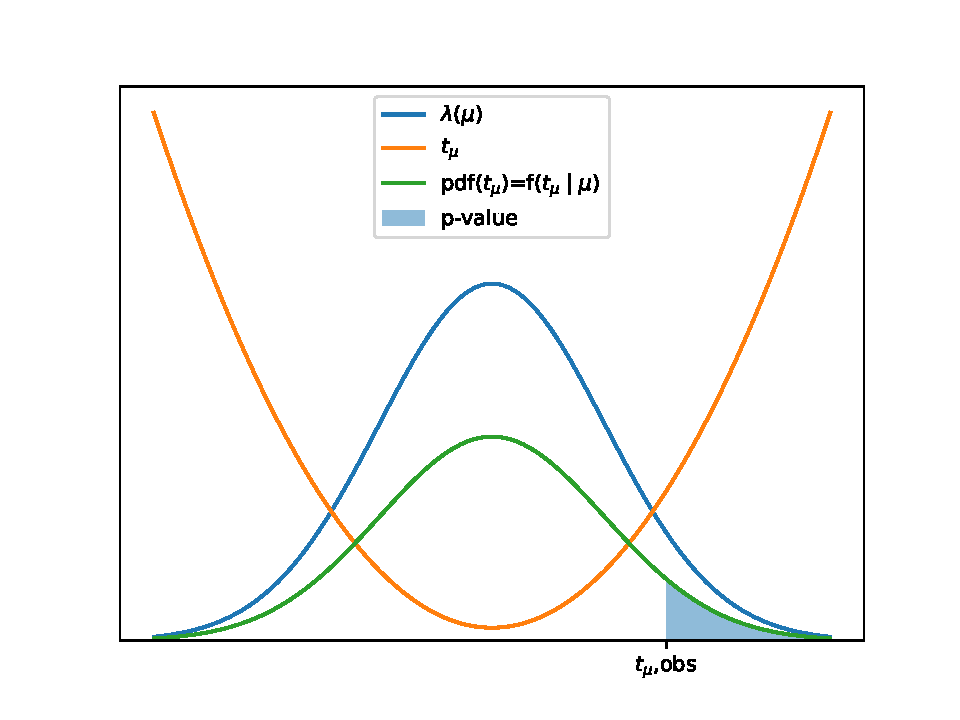
\includegraphics[width=0.8\textwidth]{test_stat_example.pdf}
    \caption[]{A sketch to follow the steps to calculate p-values. (\textbf{left}) The profile likelihood ({\color[HTML]{1f77b4}{$\bm{\diagup}$}}) has essentially some hill-like form with a maximum at ${\lambda(\hat{\mu},\hat{\bm{\Theta}})}$. The test statistic $t$ ({\color[HTML]{ff7f0e}{$\bm{\diagup}$}}) is calculated as $-2\mathrm{ln}(\lambda)$. (\textbf{right}) For one parameter of interest in the large sample limit $f(t | \mu)$ from equation \ref{eq:chi-square} follows a non-central chi-squared distribution with one degree of freedom. The blue shaded area under the probability density functions is a right hand sided p-value.}
    \label{fig:test_stat_example}
\end{figure}

The capability to compute p-values allows to state how likely it is that the proposed hypothesis is reflected by the observed data. Specifically, the p-value indicates how probable it is to obtain data at least as extreme as the observed ones if the experiment were repeated many times. This measure thus reflects the degree of incompatibility between prediction and observation.

In the scientific community a p-value of 0.05 is commonly accepted as significant. However particle physicists usually transform the p-value is into a significance via the inverse cumulative distribution function of the standard normal distribution
\begin{equation}
    Z = \Phi^{-1}(1 - p).
\end{equation}
The found p-value is thus expressed in terms of the number of standard deviations this p-value would have if the test statistic were standard normal distributed. Particle physicists only claim discovery of a new phenomenon for $Z>5$ ($p$ < \qty{2.87e-7}{}) and exclude hypotheses for $Z>2$ ($p$ < 0.05). When setting data points to the expected number of events predicted by the model an estimate for the significance can be calculated referred to as Asimov significance from the bin contents
\begin{equation}\label{eq:asimov-significance}
    Z_A = \sqrt{2\sum_{i\in bins}((s_i + b_i)(\log{(1 + s_i / b_i)}) - s_i)}.
\end{equation}


A key consideration is that $t$ can assume negative values for $\mu$ which might be non-physical depending on the context. This is handled by cutting off the test statistic for undesired behavior. An example of an adjusted test statistic for setting upper limits is
\begin{equation}
    q_\mu=
    \begin{cases}
        -2\ln \lambda(\mu) & \hat{\mu}\leq\mu \\
        0                  & \hat{\mu}> \mu
    \end{cases}.
\end{equation}
Here, if a tested signal strength $\mu$ is not larger than the maximum estimate, it would not be regarded as less compatible and is therefore set to zero. Various cases and approximations of probability density functions in different scenarios are detailed in \citep{cowan2011asymptotic}.

\section{The CL$_s$ Value}\label{sec:cls}
Particle physicists typically concentrate on two key aspects when performing statistical tests to discover new phenomena: the accurate modeling of known backgrounds and whether there is evidence in the observations for a new phenomenon. This involves assessing two distinct hypotheses: a background only ($b$) and one that involves signal and background ($s+b$). Each will result in a p-value of their own.

To combine these two aspects into a unified metric particle physicists developed the CL$_s$ quantity. This measure not only considers the potential presence of new phenomena but also the accuracy of the background modeling.
\begin{equation}
    \mathrm{CL}_s=\frac{p_{s+b}}{1-p_{b}}=
    \frac
    {\int_{t_\text{obs}}^{\infty}
        f(t_{s+b} | \mu) \mathrm{d}t}
    {1-\int_{t_\text{obs}}^{\infty}
        f(t_{b} | \mu) \mathrm{d}t}.
\end{equation}
The numerator represents the p-value for the alternative hypothesis while the denominator penalizes the $p_{s+b}$ based on how compatible the background model is with the observational data. For example, $p_{b} = 0$ would indicate a perfect modeling of backgrounds. This becomes particularly useful in searches with poor sensitivity as the hypothesis test depends crucially on the background estimate. The concept can also be understood visually from the first figure of the paper that introduced the CL$_s$ quantity \citep{read2002presentation} and is explained here in figure \ref{fig:cls}.
\begin{figure}
    \centering
    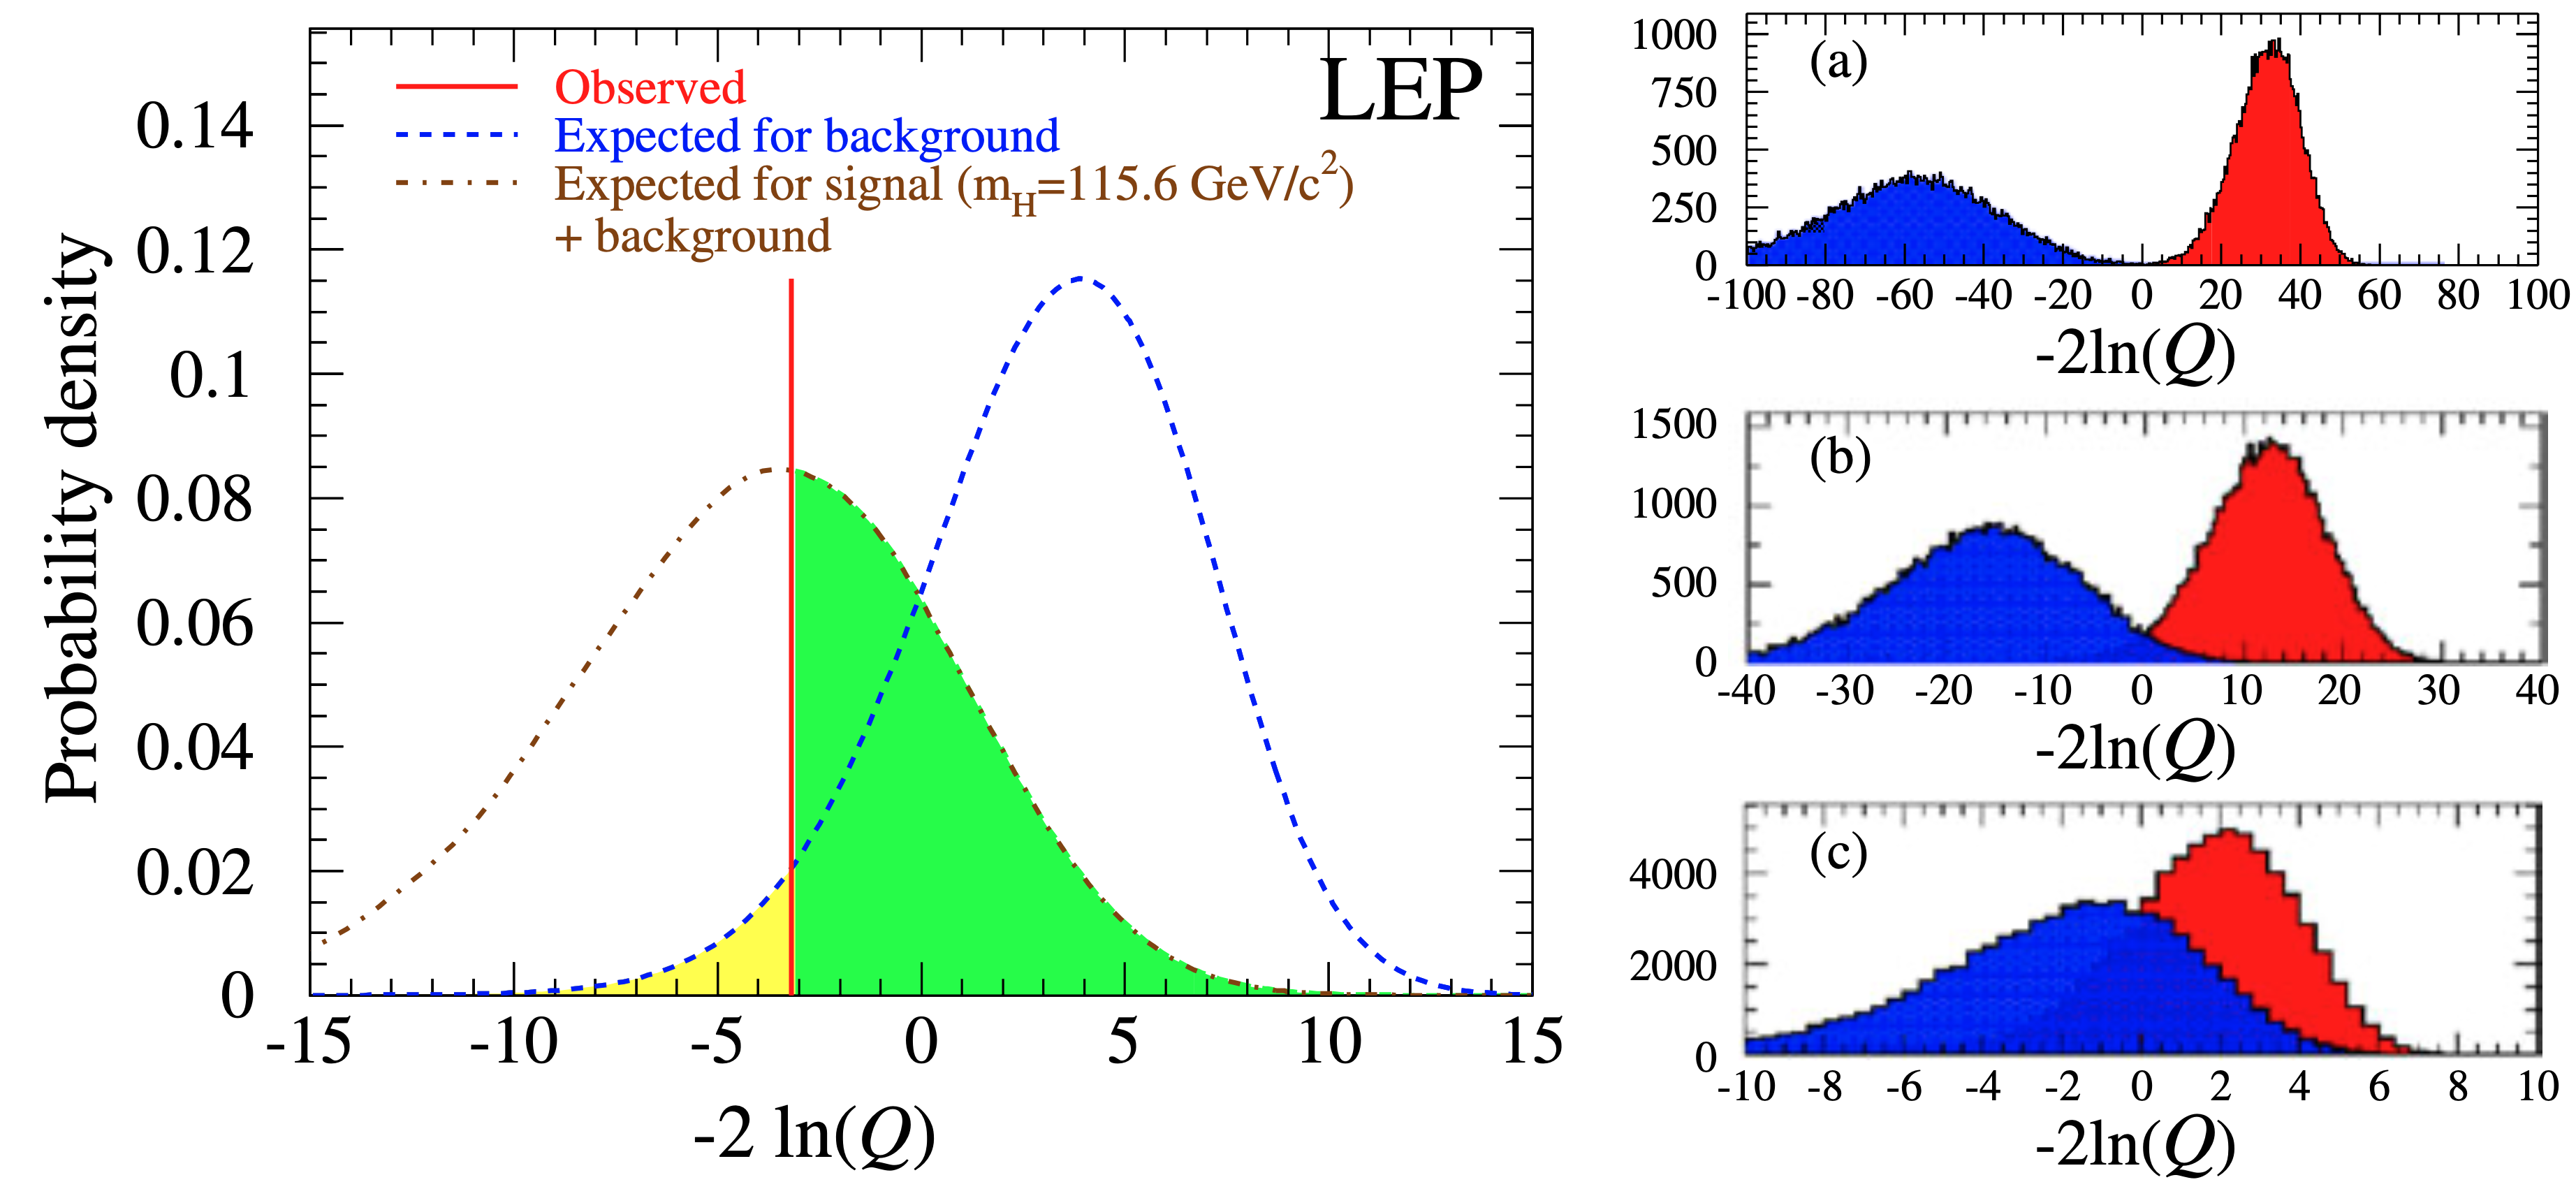
\includegraphics[width=1\textwidth]{cls.png}
    \caption[]{Probability density functions of test statistics from a Higgs search at LEP illustrating the calculation of p-values ($\lambda$ from the full text becomes $Q$). (\textbf{left}) The probability density functions of the test statistic $f(t | \mu)$ of the signal + background ({\color[HTML]{804000}{$\bm{\diagup}$}}) and background ({\color[HTML]{2100FF}{$\bm{\diagup}$}}) only hypotheses. The p-value is calculated by integration from $t_\text{obs}$ (the red observed line ({\color[HTML]{FF0000}{$\bm{\diagup}$}})) to infinity (see eq. \ref{eq:p-value}). The green shaded area (\hexbox{00FF00}) corresponds to $p_{s+b}$ whereas the yellow area (\hexbox{FDFF02}) corresponds to $1-p_b$ since the integral over one whole probability density is 1. (\textbf{right}) Degradation of search sensitivity from (a) to (c). Note that the colors of the probability density functions change here to signal + background (\hexbox{2100FF}) and background only (\hexbox{FF0000}). For example putting the observation ($t_\text{obs}$) on the x-axis at 0 in these plots, one would get for plot (a) $p_{b}\approx 1$ and $p_{s+b}\approx 0$ resulting in a CL$_s\approx 0$, whereas with increasing overlap the CL$_s$ value increases and the sensitivity decreases. Adopted from \citep{read2002presentation}.}
    \label{fig:cls}
\end{figure}


\red{test statistic: want to check if we can reject what we are testing on}
\red{constraint term is a penalty for a pull}


\section{HistFactory}\label{sec:histfactory_model}
A widely-used model for constructing likelihoods as discussed in section \ref{sec:likelihood} is known as HistFactory \citep{cranmer2012histfactory}. HistFactory simplifies the process of building a likelihood by breaking it down into several fundamental components. This considers a different categorization of the model parameters $\bm{\phi}$
\newcommand{\freeset}{\bm{\eta}}
\newcommand{\constrset}{\bm{\chi}}
\newcommand{\singleconstr}{\chi}
\newcommand{\channelcounts}{\bm{n}}
\newcommand{\auxdata}{\bm{a}}
\newcommand{\poiset}{\bm{\psi}}
\newcommand{\nuisset}{\bm{\theta}}
\newcommand{\fullset}{\bm{\phi}}
\newcommand{\singlefull}{\phi}
\begin{equation}
    L(\bm{x}|\fullset) \quad=\quad
    L(\bm{x}|\overbrace{\poiset}^{\llap{\text{parameters of interest}}},\underbrace{\nuisset}_{\llap{\text{nuisance parameters}}}) \quad=\quad
    L(\bm{x}|\overbrace{\freeset}^{\rlap{\text{free}}},\underbrace{\constrset}_{\rlap{\text{constrained}}}),
\end{equation}
into free parameters $\freeset$ and constrained parameters $\constrset$ which are used to incorporate uncertainties into the likelihood to constrain it. Further there might be several histograms of an observable, for example measured in orthogonal kinematic regions, that are called channels $c$. Bins have the index $b$ here and constraint terms are denoted $c_{\singleconstr}$. The likelihood can thus be described by
\begin{equation}
    L(\channelcounts, \auxdata \,|\,\freeset,\constrset)
    = \underbrace{{\prod_{c\in\mathrm{\,channels}} \prod_{b \in \mathrm{\,bins}_c}
                \textrm{Pois} (
                \;\overbrace{n_{cb}}^{\llap{\text{\strut observed}\quad\;}}
                \,|\, \overbrace{\nu_{cb}\left(\freeset,\constrset\right)}^{\llap{\quad\text{\strut predicted}}}
                \;)}}_{\substack{\text{Simultaneous measurement}\\%
            \text{of multiple channels}}}
    \underbrace{{\prod_{\singleconstr \in \constrset} c_{\singleconstr}(a_{\singleconstr} |\, \singleconstr)}}_{\substack{\text{constraint terms}\\%
            \text{for }\text{auxiliary measurements}}}.
    \label{eq:histfactory_likelihood}
\end{equation}
$\bm{n}$ are observed and $\bm{a}$ the auxiliary measurement histograms. The $n_{cb}$ enter the Poisson term per bin and channel where the predicted counts per bin are governed by the free and constrained parameters $\nu_{cb}(\freeset,\constrset)$. $c_{\singleconstr}(a_{\singleconstr} |\, \singleconstr)$ are functions that penalize the likelihood $L$ with uncertainties $a_\chi$ to constrain the parameter $\singleconstr$ and are discussed in detail section \ref{sec:constraint_terms}.

The prediction is a sum of nominal counts per bin $\nu_{scb}^0$ over all samples $s$ (e.g. $t\overline{t}$, multijet-background, etc.). Counts per bin are also called rates, like in the definition of a Poisson distribution. These nominal bin counts are subject to uncertainties and have thus have some degree of freedom. However the effect of this modification to the likelihood must be taken into account which is through the constraint terms. These penalize the likelihood proportional to the modification. Modifiers are discussed in detail in section \ref{sec:modifiers}. They enter the likelihood through linear modeling of the nominal bin content $\nu_{scb}^0$ with multiplicative $\kappa_{scb}$ and additive modifiers $\Delta_{scb}$
\begin{align}
    \nu_{cb}\left(\freeset,\constrset\right) & = \sum_{s\in\mathrm{\,samples}} \nu_{scb}\left(\freeset,\constrset\right)                                                                                                \\
                                             & = \sum_{s\in\mathrm{\,samples}}\underbrace{\left(\prod_{\kappa\in\,\bm{\kappa}} \kappa_{scb}\left(\freeset,\constrset\right)\right)}_{\text{multiplicative modifiers}}\,
    \Bigg(\nu_{scb}^0 + \underbrace{\sum_{\Delta\in\bm{\Delta}} \Delta_{scb}\left(\freeset,\constrset\right)}_{\text{additive modifiers}}\Bigg).
    \label{eq:modifier_equation}
\end{align}
The usefulness of this approach becomes clear when considering one uncertainty $a_\chi$ on a nominal bin count estimate $\nu_{scb}^0$. The main goal remains to maximize the overall likelihood $L$. This can be achieved via maximizing the Poisson probability (blue part in equation \ref{eq:histfactory_likelihood}) and at the same time keeping the constraint term (red part in equation \ref{eq:histfactory_likelihood}) large. It is illustrative to consider one nuisance parameter $\chi$ as a multiplicative modifier $\kappa_{scb}=\chi$ on $\nu_{scb}^0$. An optimum can be found by modifying the prediction to move closer to the observed value while at the same time keeping the constraint term controlled by the same $\chi$ at values where the penalization of the likelihood stays insignificant. This works well for example when $\kappa$ has a very large uncertainty rendering the constraint term's influence on the likelihood relatively small.

\subsection{Modifiers}\label{sec:modifiers}
In HistFactory there are by convention four types $\{\lambda,\mu,\gamma,\alpha\}$ of such multiplicative rate modifiers that are explained in this section. There are \textbf{free rate modifiers} for the luminosity $\lambda$ and signal strength $\mu$ that affect all bins equally
\begin{equation}
    \nu_{scb}(\mu)=\mu \nu_{scb}^0.
\end{equation}
These are bin-independent normalization factors and preserve the shape of the histogram.
Further there are \textbf{bin-wise modifiers} $\gamma_b$ (uncorrelated shape)
\begin{equation}
    \nu_{scb}(\gamma_b)=\gamma_b \nu_{scb}^0.
\end{equation}
These are useful for example to include uncertainties of a per bin data-driven background estimate. This type without a constraint term is not of much use as if there is only one sample or channel, the fit would always match the data perfectly.
In addition there exist \textbf{interpolation parameters $\alpha$} (shape factors) that enter the modeling through an interpolation function $\eta$ instead of being the factor itself. They exist in multiplicative versions
\begin{equation}
    \nu_{scb}(\alpha)=\eta(\alpha) \nu_{scb}^0,
\end{equation}
and additive versions
\begin{equation}
    \nu_{scb}(\alpha)=\nu_{scb}^0 + \eta(\alpha).
\end{equation}
This is useful to include systematic uncertainties. Typically they are known for one standard deviation of count in a bin $\eta_{-1}=\nu_{scb}^\mathrm{1down}$ and $\eta_{1}=\nu_{scb}^\mathrm{1up}$ to the nominal value $\nu_{scb}^0$. These are then used to construct interpolation functions that modify the nominal value controlled by the nuisance parameter and also control the constraint term $c_\alpha$, further explained in section \ref{sec:constraint_terms}, such that one parameter controls the modification and constraint at a time.

In HistFactory there exists four of such interpolation functions. For those exist an identity operator
\begin{equation}
    \eta_0=\eta (\alpha=0) =
    \begin{cases}
        1 , & \text{multiplicative modifier, } (\kappa) \\
        0 , & \text{additive modifier, } (\lambda).
    \end{cases}
\end{equation}
One example of these interpolation functions that scales the count in a bin linearly over the known deviations $\eta_{-1}=\nu_{scb}^\mathrm{1down}$ and $\eta_{1}=\nu_{scb}^\mathrm{1up}$ is
\begin{equation}
    \eta_\mathrm{linear}(\alpha)=
    \begin{cases}
        \alpha(\eta_0 - \eta_1) ,    & \alpha>0 \\
        \alpha(\eta_0 - \eta_{-1}) , & \alpha<0
    \end{cases}
\end{equation}
This is illustrated in fig. \ref{fig:interp_func}(a). For the other ones see e.g. \citep{heinrich2019searches}. It is noted that $\alpha$ is the nuisance parameter and not the function $\eta(\alpha)$ and there is an associated constraint term $c_\alpha$ to each $\alpha$.
\begin{figure}
    \centering
    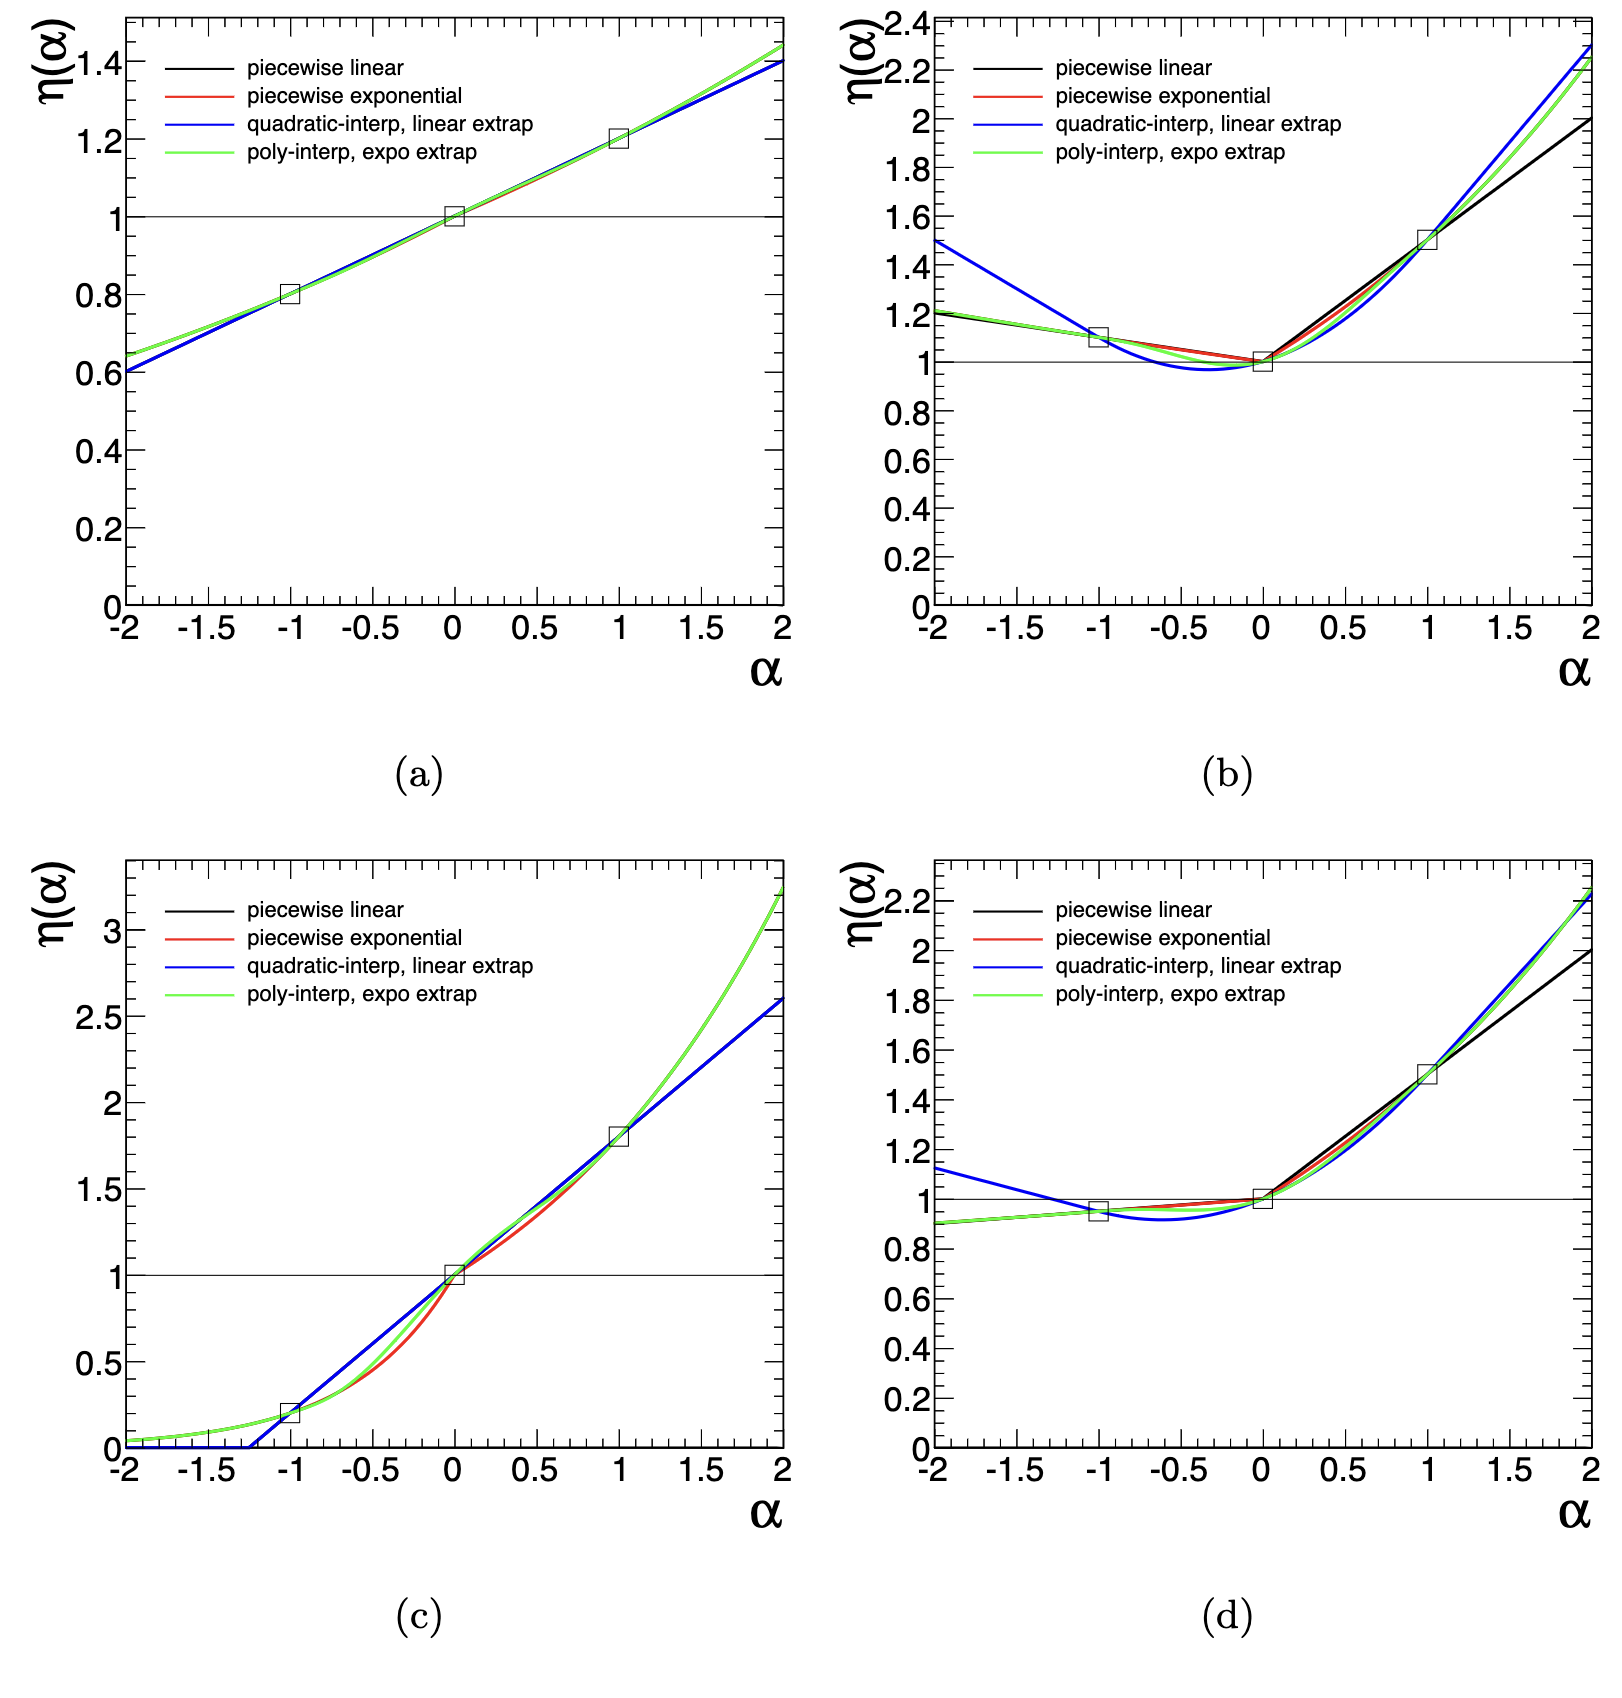
\includegraphics[width=.8\textwidth]{interp_func.png}
    \caption[]{The four interpolation functions $\eta(\alpha)$ for different up and down standard deviation values. For example in (a) the bin count will be scaled with a factor of 0.8 for an $\alpha=-1$ (1.2 for an $\alpha=1$). From \citep{cranmer2012histfactory}.}
    \label{fig:interp_func}
\end{figure}

\subsection{Constraint Terms}\label{sec:constraint_terms}
Uncertainties are modeled either Gaussian or Poissonian. The Gaussian uncertainty implementation is straightforward as the standard deviation $\sigma$ appears in the definition of the Gaussian with mean $\mu$
\begin{equation}
    \text{Gaus}(\mu|x,\sigma)=\frac{1}{\sigma\sqrt{2\pi}}e^{-\frac{1}{2}\left(\frac{x-\mu}{\sigma}\right)^2}.
\end{equation}
So that the likelihood for a Gaussian uncertainty is constrained by a Gaussian scaled to one standard deviation controlled by the nuisance parameter $\alpha$: \mbox{$\mathrm{Gauss}(\alpha | a, \sigma=1)$}.

The Poisson distribution reads
\begin{equation}
    \text{Pois}(k|r)= \frac{r^k e^{-r}}{k!}.
\end{equation}
For a Poissonian distributed uncertainty the nuisance parameter for a multiplicative factor $\kappa_{scb}=\gamma$ in equation \ref{eq:modifier_equation} should control the Poisson constraint term such that the uncertainty $\sigma$ is reflected by the variance of the Poisson $\text{Var}(\text{Pois})=r=\sigma^2$. This is achieved by scaling the distribution with a factor $f$ which is then solved for the one with the desired uncertainty by evaluating it at the nominal value of the multiplicative modifier $\gamma_0=1$
\begin{equation}
    \mathrm{Var}\left[\mathrm{Pois}(k=f\gamma_0 | r=f\gamma)\right]
    =
    r=f\gamma\;\stackrel{\gamma=\gamma_0}{=}\;f\gamma_0=(f\sigma)^2
    \quad
    \rightarrow \quad f=(1/\sigma^2).
\end{equation}
Thus a Poissonian constraint term for a multiplicative modifier $\gamma$ with uncertainty $\sigma$ reads \mbox{$\text{Pois}(k=\sigma^{-2}|r=\sigma^{-2}\gamma)$.} This completes the necessities for the HistFactory model. The different types of modifiers and their constraint terms are summarized in table \ref{tab:histfactory}.
\begin{table}[]
    \caption[]{Modifiers and constraint terms used by HistFactory. Note that the interpolation functions are called $f_p$ and $g_p$ here instead of $\eta$ as chosen in the full text. Input for the constraint terms are the corresponding uncertainties. Adapted from \citep{pyhf}.}
    \centering
    \resizebox{0.97\textwidth}{!}{
        \begin{tabular}{l|l|l|l}\label{tab:histfactory}
            Description          & Modification                                                                                            & Constraint Term $c_\singleconstr$                                                            & $c_\chi$ input                     \\
            \hline
            Uncorrelated Shape   & $\kappa_{scb}(\gamma_b) = \gamma_b$                                                                     & $\prod_b \mathrm{Pois}\left(k_b = \sigma_b^{-2}\middle|\,r_b = \sigma_b^{-2}\gamma_b\right)$ & $\sigma_{b}$                       \\
            Correlated Shape     & $\Delta_{scb}(\alpha) = f_p\left(\alpha\middle|\,\Delta_{scb,\alpha=-1},\Delta_{scb,\alpha = 1}\right)$ & $\displaystyle\mathrm{Gaus}\left(a = 0\middle|\,\alpha,\sigma = 1\right)$                    & $\Delta_{scb,\alpha=\pm1}$         \\
            Normalisation Unc.   & $\kappa_{scb}(\alpha) = g_p\left(\alpha\middle|\,\kappa_{scb,\alpha=-1},\kappa_{scb,\alpha=1}\right)$   & $\displaystyle\mathrm{Gaus}\left(a = 0\middle|\,\alpha,\sigma = 1\right)$                    & $\kappa_{scb,\alpha=\pm1}$         \\
            MC Stat. Uncertainty & $\kappa_{scb}(\gamma_b) = \gamma_b$                                                                     & $\prod_b \mathrm{Gaus}\left(a_{\gamma_b} = 1\middle|\,\gamma_b,\delta_b\right)$              & $\delta_b^2 = \sum_s\delta^2_{sb}$ \\
            Luminosity           & $\kappa_{scb}(\lambda) = \lambda$                                                                       & $\displaystyle\mathrm{Gaus}\left(l = \lambda_0\middle|\,\lambda,\sigma_\lambda\right)$       & $\lambda_0,\sigma_\lambda$         \\
            Normalisation        & $\kappa_{scb}(\mu_b) = \mu_b$                                                                           &                                                                                              &                                    \\
            Data-driven Shape    & $\kappa_{scb}(\gamma_b) = \gamma_b$                                                                     &                                                                                              &                                    \\
        \end{tabular}
    }
\end{table}



\section{Uncertainty Extraction}
The standard error of a quantity is determined by measuring the square root of its variance. The covariance matrix is a generalization of variance for two random variables $X_i, X_j$
\begin{equation}
    \Sigma_{ij}=\text{Cov}(X_i, X_j) = \text{E}[(X_i - \text{E}[X_i])(X_j - \text{E}[X_j])].
\end{equation}

In the context of maximum likelihood estimation, the covariance matrix of the nuisance parameters \( \bm{\theta} \) can be approximated in the large sample limit by the inverse of the negative Hessian of the log-likelihood function $L$

\begin{equation}
    \Sigma_{ij} \approx \left[ -\frac{\partial^2 L(\bm{\theta})}{\partial \theta_i \partial \theta_j} \right]^{-1}.
\end{equation}

The covariance matrix holds the variances and thus the uncertainties of the nuisance parameters along its diagonal, and the covariances between components off-diagonal. When propagating uncertainties, these covariances contribute to the overall uncertainty. Consequently, large correlations between parameters, indicated by large off-diagonal terms, are thus disadvantageous for constraining the model.
